\documentclass{article}

\usepackage[utf8]{inputenc}
\usepackage[T1]{fontenc}
\usepackage[greek,english]{babel}
\usepackage{alphabeta}
\usepackage{amsmath}
\usepackage{amssymb}
\usepackage{graphicx}
\usepackage{subcaption}
\usepackage{epstopdf}
\usepackage[margin=1in, paperwidth=7.5in,paperheight=10.5in]{geometry}


\newcommand\course{ΤΗΛ513}
\newcommand\courseName{Δορυφορικές Ζεύξεις}
\newcommand\semester{Εαρινό 2020}
\newcommand\assignmentNumber{Lab 5 Δορυφορικών Επικοινωνιών}
\newcommand\studentName{Μαυρογιώργης Δημήτρης}                           
\newcommand\studentNumber{2016030016}

\title{\underline{\textbf{\assignmentNumber}}} 
\author{\textsc{\textbf{Όνομα:}}  \studentName\\
		\textsc{\textbf{ΑΜ:}}  \studentNumber\\
		\course \ - \courseName\\ 
		\textsc{Πολυτεχνείο Κρήτης}
}
\date{\today}
\begin{document}
	\maketitle
\section{Εισαγωγή}
Σκοπός της συγκεκριμένης άσκησης είναι να δούμε τον τρόπο λήψης, επεξεργασίας και εξαγωγής πληροφορίας από δορυφορικό σήμα. Πιο συγκεκριμένα, έγινε λήψη και επεξεργασία σήματος από το δορυφόρο Meteor M-N2.\\

\noindent
Αρχικά, έχοντας δωθεί το αρχείο(.wav) με το ληφθέν σήμα από το δορυφόρο, χρησιμοποιήθηκαν κάποια προγράμματα για την αποδιαμόρφωση και την εμφάνιση της εικόνας που μας έστειλε ο δορυφόρος. Τα προγράμματα αυτά ήταν το SDRSharp και το LRPT Decoder. Επιπλέον, για τη βελτίωση της ποιότητας της εικόνας έγινε η χρήση του προγράμματος Smooth Meteor.\\

\noindent
Για την offline αποδιαμόρφωση του σήματος, φορτώθηκε το αρχείο .wav στο SDRSharp και αφού ρυθμίστηκαν κατάλληλα οι παράμετροι τις αποδιαμόρφωσης του σήματος, όπως π.χ. το bandwidth, modulation type, ρυθμός μετάδοσης κ.λ.π.\\

\noindent
Έπειτα από μερικά λεπτά, αφού ολοκληρώθηκε η διαδικασία της αποδιαμόρφωσης με το SDRSharp, προέκυψε ένα αρχείο .s, το οποίο δώθηκε ως είσοδος στο πρόγραμμα LRPT Decoder. Το συγκεκριμένο πρόγραμμα χρησιμοποιήθηκε για την εμφάνιση της εικόνας που μας έστειλε ο δορυφόρος. Επιπροσθέτα, η εικόνα που προέκυψε επεξεργάστηκε μέσω του προγράμματος Smooth Meteor, με το οποίο έγινε ομαλοποίηση των χρωμάτων. Τα αποτελέσματα που προέκυψαν από τη συνολική λήψη και επεξεργασία του σήματος φαίνονται παρακάτω.  


\begin{figure}[h!]
	\centering
	\begin{subfigure}[t]{\textwidth}
		\centering
		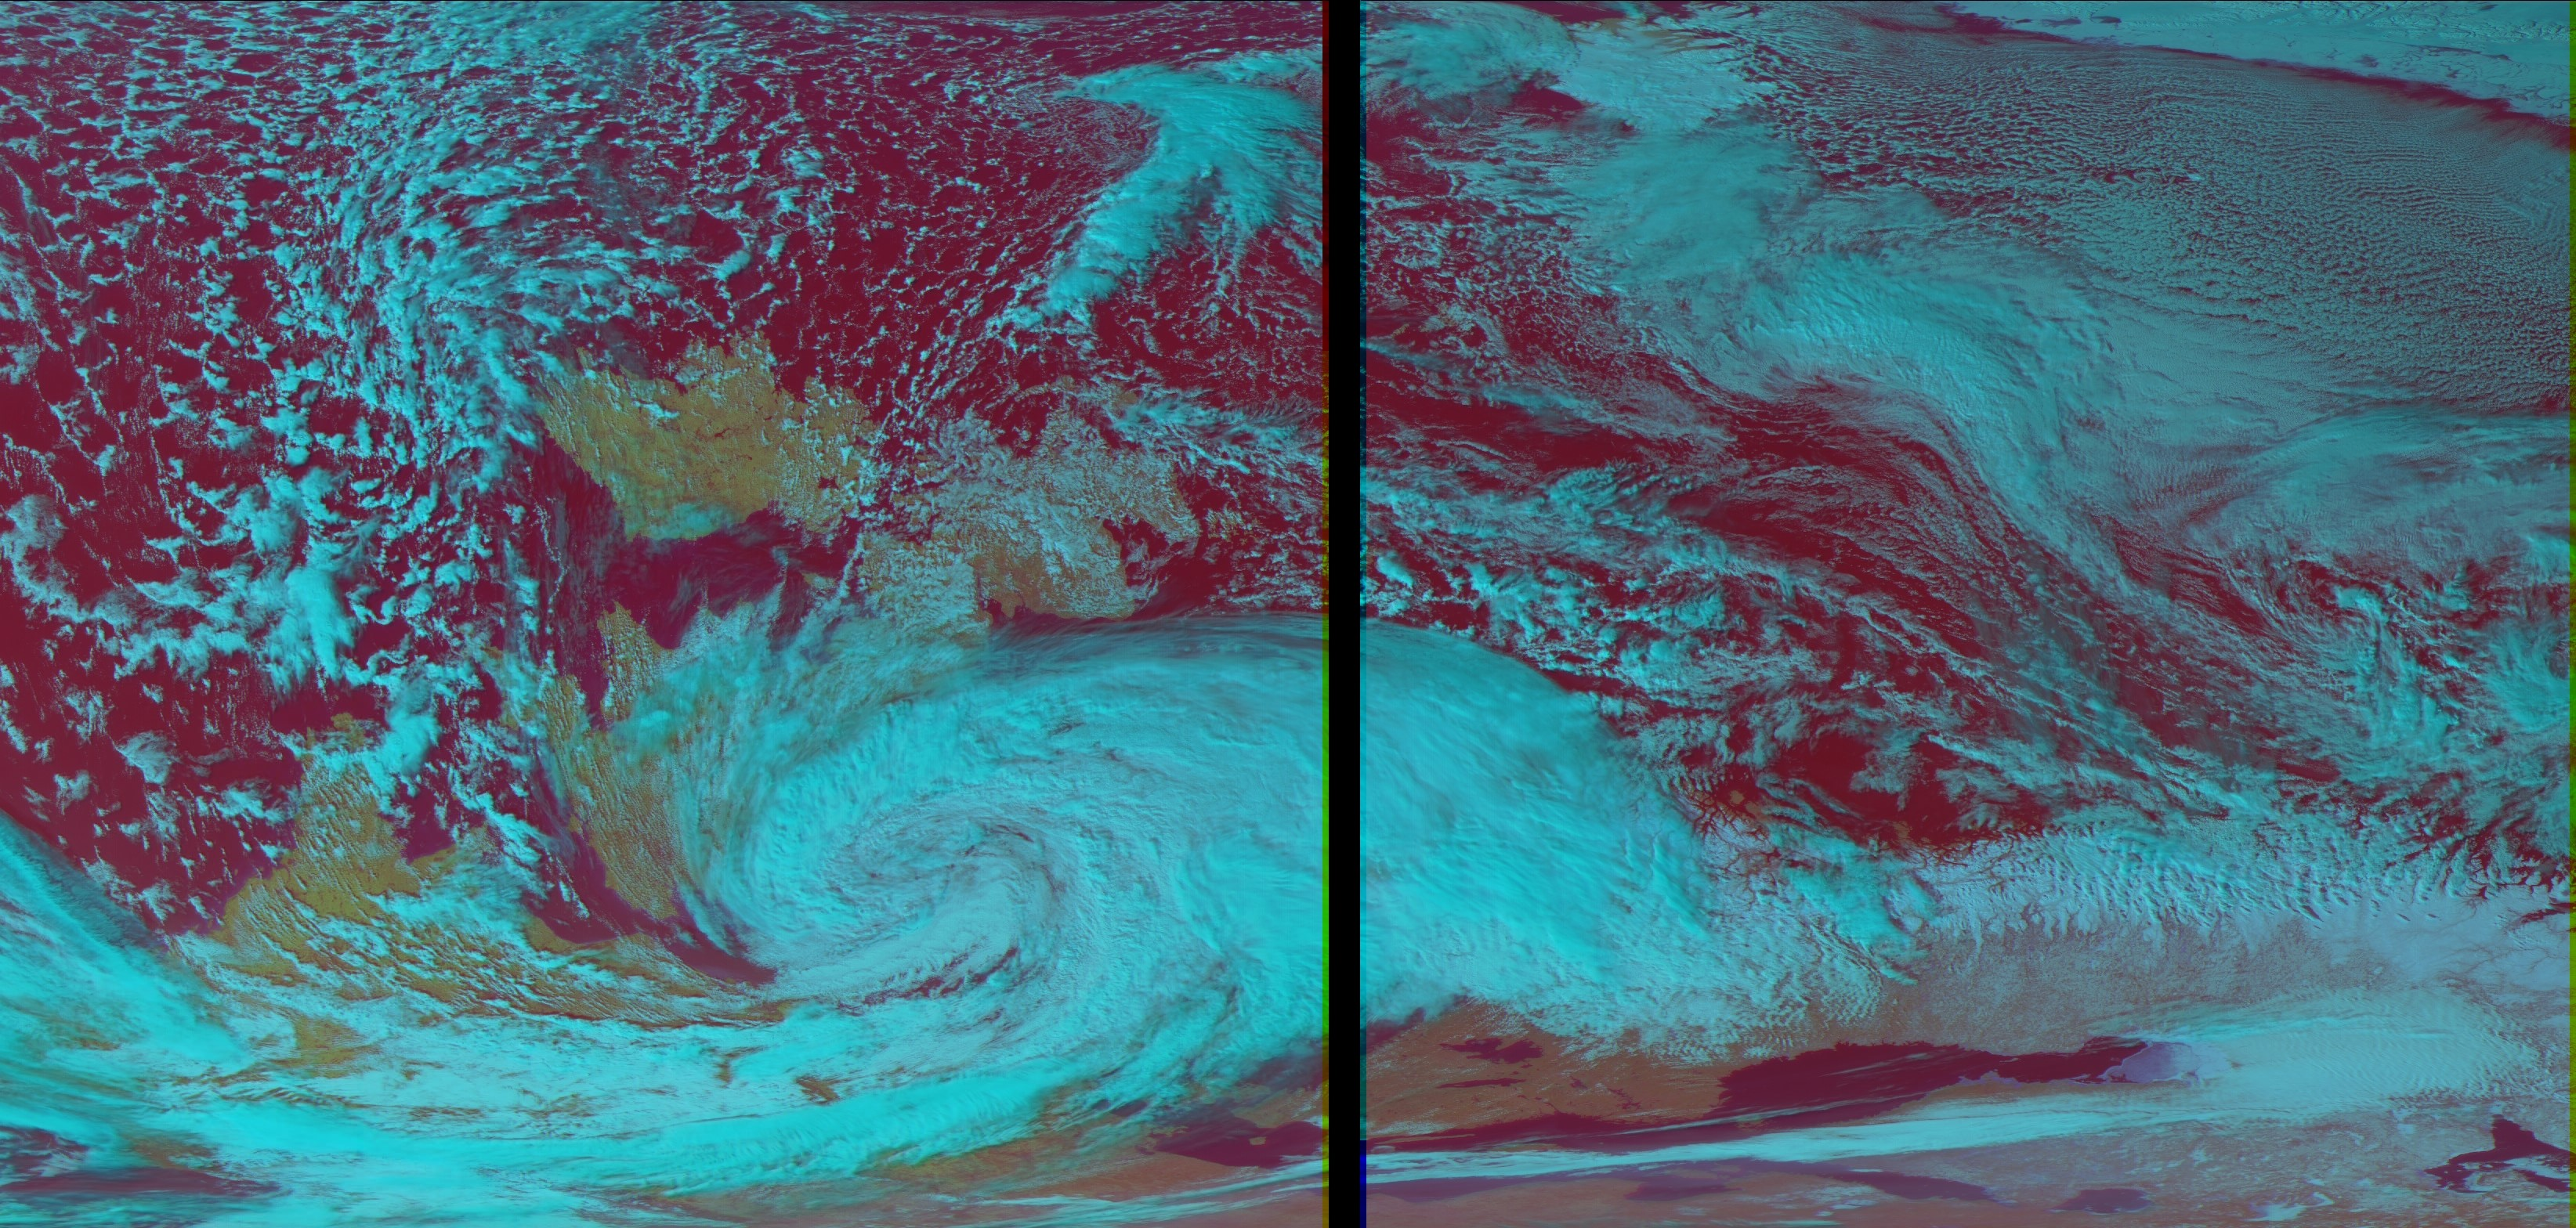
\includegraphics[width=\linewidth]{./results/meteor_img.jpg}
		\caption{Eικόνα μετά την αποδιαμόρφωση(SDRSharp) και εμφάνιση (LRPT Decoder)}
	\end{subfigure}
	~
	\begin{subfigure}[t]{\textwidth}
		\centering
		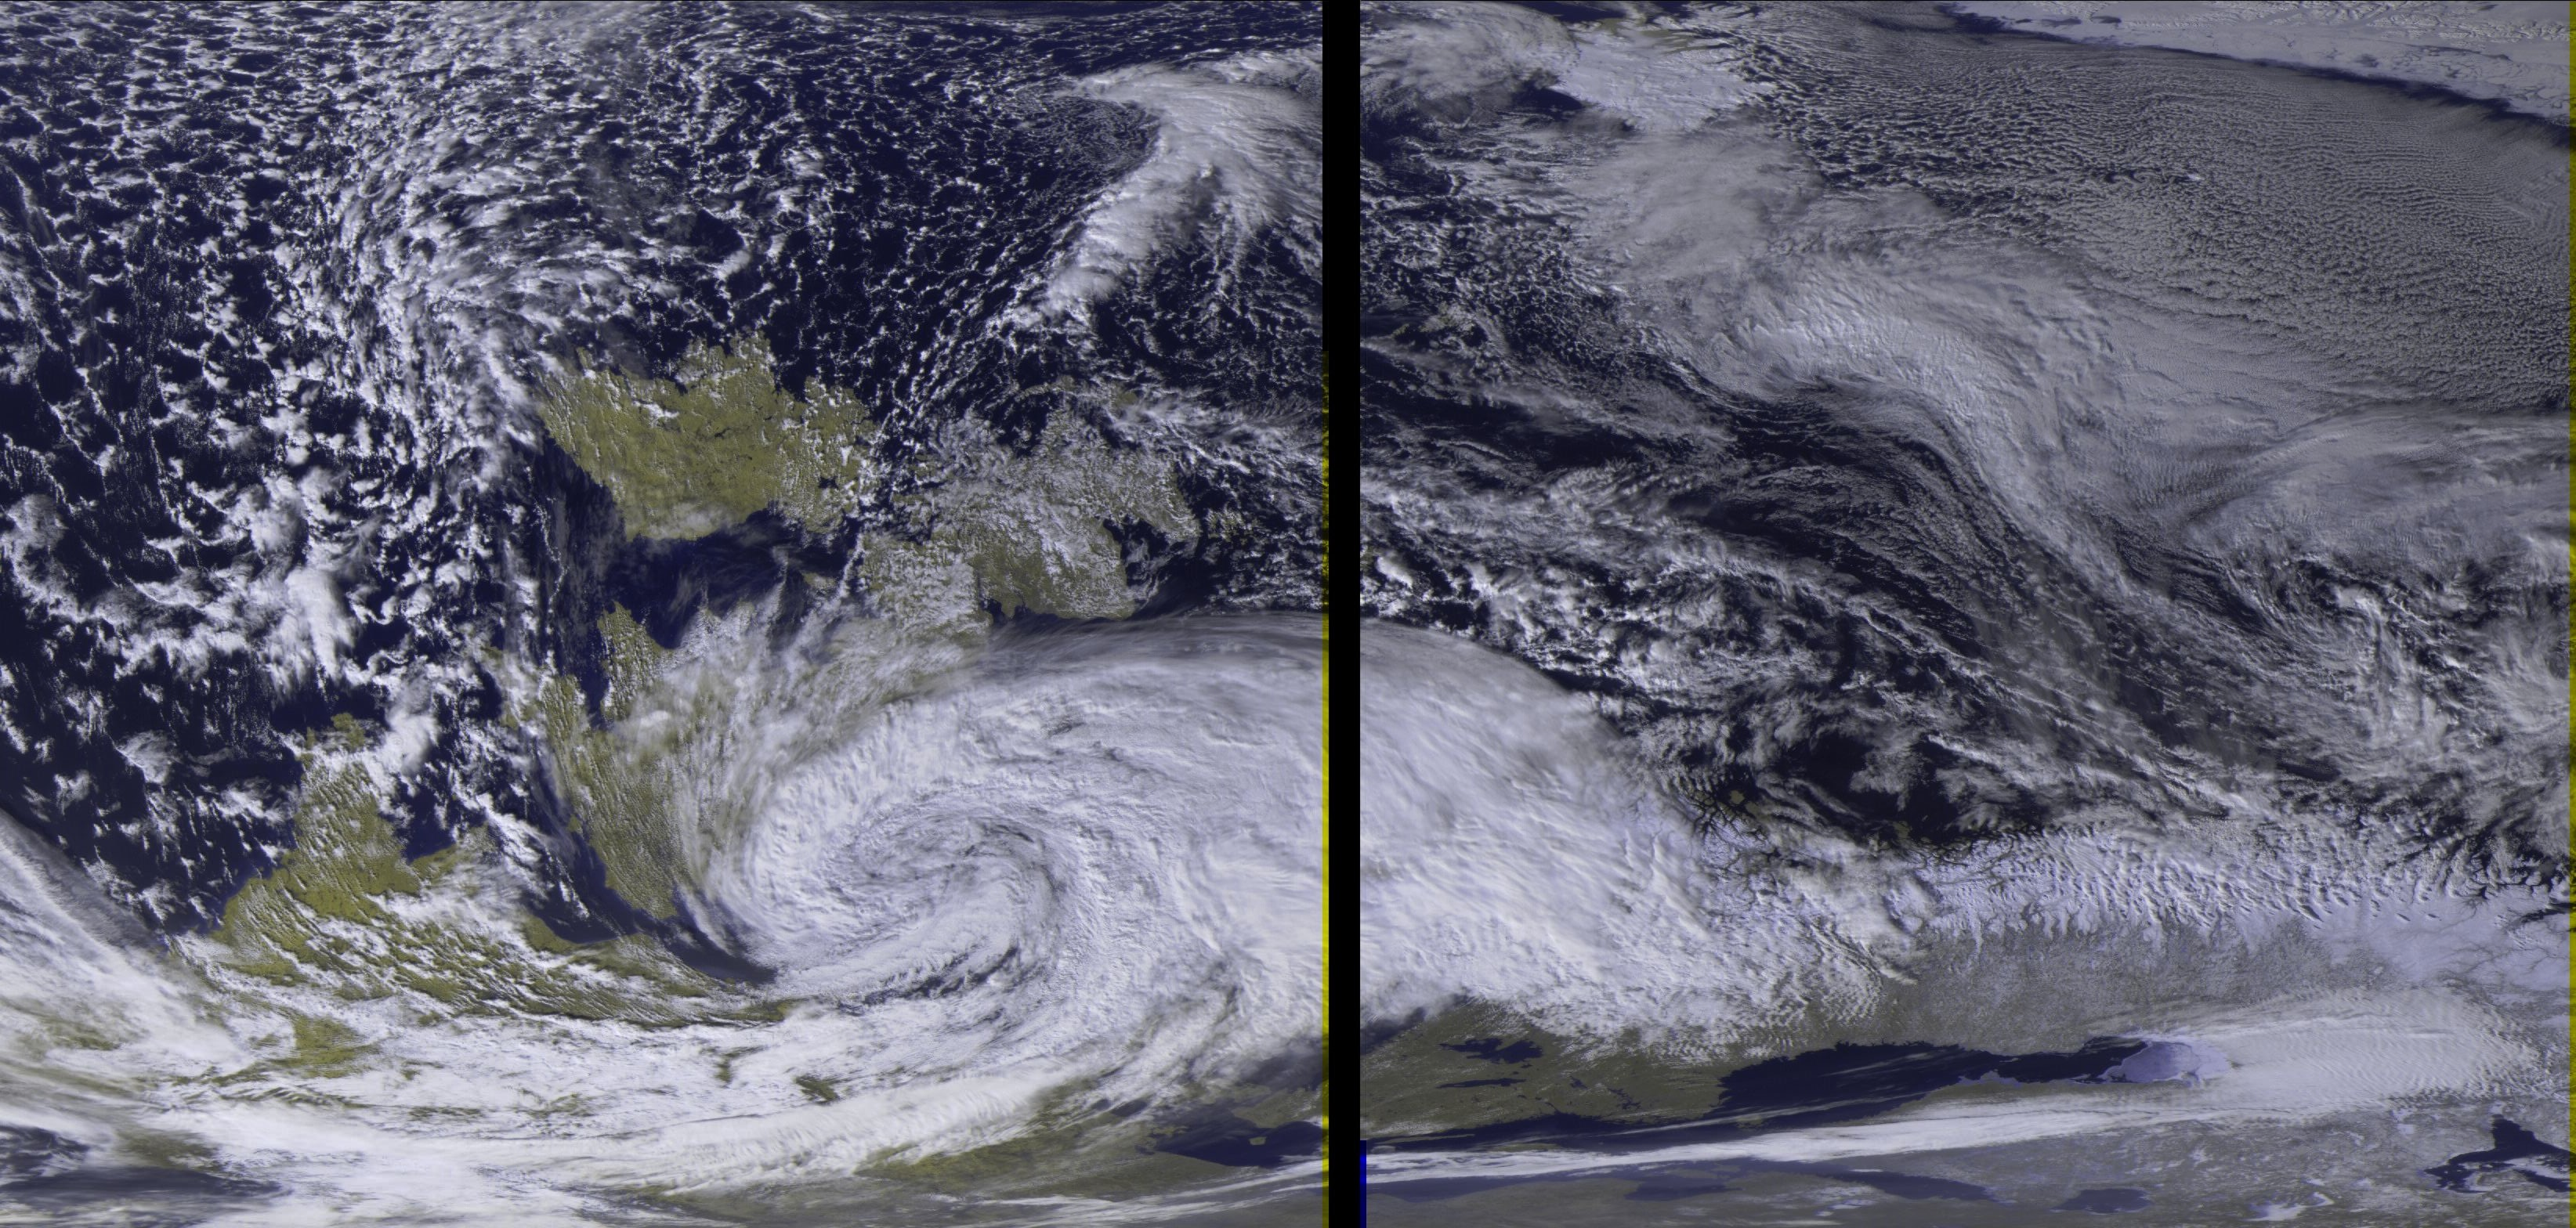
\includegraphics[width=\linewidth]{./results/meteor_smooth_img.jpg}
		\caption{Eικόνα μετά την επεξεργασία με το  Smooth Meteor}
	\end{subfigure}
\end{figure}
\pagebreak
\section{Eρώτημα 1}
Στόχος του πρωτοκόλλου NTP (Network Time Protocol) είναι να παρέχει ένα ή περισσότερα σημεία αναφοράς για ώρα υψηλής ακριβείας. Η περιορισμένη ακρίβεια των ρολογιών των δικτυακών συσκευών επιβάλει τον συγχρονισμό τους σε τακτά χρονικά διαστήματα με κάποια ώρα αναφοράς υψηλής ακρίβειας. Η ρύθμιση λοιπόν των ρολογιών στις συσκευές του δικτύου γίνεται με χρήση του συγκεκριμένου πρωτοκόλλου. Επομένως, είναι απαραίτητη η σύνδεση του λογισμικού σε έναν εξυπηρετητή NTP, ώστε να συγχρονιστεί το ρολόι του λογισμικού με βάση το παγκόσμιο ρολόι και έτσι να μπορούμε να κάνουμε track το δορυφόρο.

\pagebreak
\section{Eρώτημα 2}
Aπό ένα Two Line Element(TLE) μπορούμε να πάρουμε πληροφορία γενικές πληροφορίες για τον δορυφόρο (Αριθμός καταλόγου, χρονολογία εκτόξευσης κ.λ.π), καθώς και χρήσιμη πληροφορία για την τροχίά του δορυφόρου. Ειδικότερα, η πληροφορία που αντλούμε για την τροχιά του(2η γραμμή του TLE) είναι η εξής:\\

\noindent
Ορθή άνοδος του ανοδικού κόμβου(Right Ascension of the Ascending Node), Κλίση(Inclination), όρισμα περιγείου(Argument of Perigee), Εκκεντρότητα (Eccentricity), Μέση ανωμαλία(Μean Anomaly) και η Μέση κίνηση (Mean motion).\\ 

\noindent
Από τα παραπάνω η ορθή άνοδος του ανοδικού κόμβου, η κλίση και το όρισμα περιγείου μας δίνουν πληροφορία για το που βρίσκεται η ελλειπτική τροχιά του δορυφόρου στο γεωκεντρικό σύστημα συντεταγμένων. Τα υπόλοιπα τρία στοιχεία μας δίνουν πληροφορία για το που βρίσκεται ο δορυφόρος πάνω στην έλλειψη. Επομένως, αν θέλουμε να υπολογίσουμε τη θέση του δορυφόρου μπορούμε να τη βρούμε με τον εξής τρόπο:\\

\noindent
Aν γνωρίζουμε τη μέση ανωμαλία μίας εβδομάδας και θέλουμε να υπολογίζουμε την τωρινή μέση ανωμαλία, θα πρεπει στην τότε μέση ανωμαλία να προσθέσουμε το γινόμενο του n(mean motion) με το Δt που διαμεσολάβησε από τότε μέχρι και τη συγκεκριμένη χρονική στιγμή τώρα ($M=n(t-t_{p}) + M_{0}$). \\

\noindent
Eπιπλέον, γνωρίζοντας την εκκεντρότητα και τη μέση ανωμαλία μπορούμε να υπολογίσουμε την εκκεντρική ανωμαλία Ε με βάση τον τύπο
$$Μ = Ε - e \ sin(E)$$

\noindent
Τέλος, από την εκκεντρική ανωμαλία μπορούμε να υπολογίσουμε την αληθή ανωμαλία με βάση τη σχέση 
$$ cos(φ_{0}) =\frac{cos(E) - e}{1 - e \ cos(E)}$$
\section{Eρώτημα 3}
Aπό την παραπάνω εικόνα που λήφθηκε από το δορυφόρο καταλαβαίνουμε ότι το μέρος του κόσμου που απεικονίζει είναι η βορειοδυτική Ευρώπη και πιο συγκεκριμένα η Αγγλία, Σκωτία και ένα μέρος της ανατολικής Γαλλίας, Βέλγιο, καθώς και κάποιες Σκανδιναβικές χώρες. 


\end{document}
